\providecommand{\main}{../../..}
\providecommand{\Figures}{\main/Figures}

\documentclass[\main/main.tex]{subfiles}

\begin{document}
                    
\section{\label{sec:modeles}ZBI pourrait être utilisée pour d'autres organismes modèles}

%
L'ensemble des algorithmes présentés précédemment ont été développés sur le \pz.
%
Bien qu'il s'agisse du modèle aquatique le plus largement utilisé en laboratoire, il n'est pas nécessairement pertinent pour l'étude de la toxicologie de composés chimiques pour l'humain, du fait de sa distance évolutive, et effectuer des tests sur plusieurs espèces semble être un moyen d'éviter d'obtenir des conclusions erronées.
%
L'adaptation des travaux présentés précédemment à d'autres modèles animaux pourrait donc être réalisée.
%
Nous allons maintenant présenter ce que ZBI pourrait apporter à l'étude des trois espèces présentées en section~\ref{sec:intro:modele}.

    \subsection{L'utilsation de ZBI sur le médaka ne demanderait que peu de modifications}

%%
%
Dans le cadre de ma thèse, j'ai essayé d'utiliser les algorithmes développés pour le recalage
et la segmentation de \pz{} de 5dpf sur des images de médakas à 10 dpf (voir section~\ref{sec:medaka}).
%
Un exemple d'application de l'algorithme de recalage est ainsi visible en Fig.~\ref{fig:model:oz:reg}.
%
Ces données restent préliminaires, car je n'ai pas pu reproduire ces expériences sur suffisamment d'échantillons provenant d'expériences indépendantes. De plus, je n'ai pas réalisé de mesures quantitatives de la précision de segmentation, par comparaison avec des segmentations manuelles.
%
L'emploi des ces algorithmes sur cet autre organisme modèle ne demanderait donc simplement qu'une validation des algorithmes de segmentation ainsi qu'une multiplication des essais pour valider la reproductibilité des résultats obtenus.

\begin{figure}[htbp]
    \centering
    \begin{subfigure}[b]{0.475\textwidth}
       \caption{
            Échantillon avant recalage
            }
       \centering 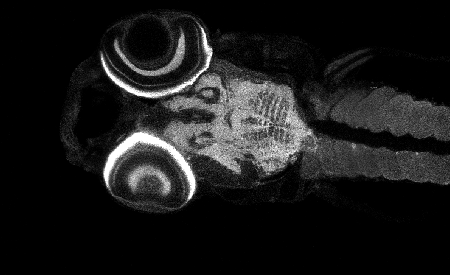
\includegraphics[width=\textwidth]{\Figures/Modeles/med_dor_raw_cut.png}
    \end{subfigure}
    \begin{subfigure}[b]{0.475\textwidth}
       \caption{
            Échantillon après recalage
            }
       \centering 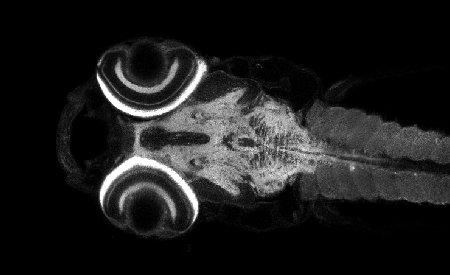
\includegraphics[width=\textwidth]{\Figures/Modeles/med_dor_reg_cut.png}
    \end{subfigure}
    \caption{
        \label{fig:model:oz:reg}
        Application du recalage à un échantillon d'\ol{}\newline
        À la vue de ce résultat, l'utilisation des algortihmes développés pour le \pz{} semble possible sans modification.
        }
\end{figure}

    \subsection{L'adaptation de ZBI au xénope nécessiterait la création de nouveaux tampons en plus d'une modification des algorithmes}
%%
%
Ces dernières années, les méthodes de clarification de tissus mises au point chez le poisson-zèbre et la souris ont été adaptées avec succès au \xl{}\cite{fini_2017,affaticati_2018}.
%
Il est donc déjà possible d'employer notre procédure d'\hti.
%
Il pourrait cependant être nécessaire de développer de nouveaux tampons afin de simplifier le montage des échantillons
tout en améliorant ainsi la robustesse de l'acquisition automatique.
%
Enfin, la forme du cerveau des têtards de \xl présentant une forte différence avec le cerveau du \pz à 5 dpf,
une adaptation des algorithmes de segmentation risque d'être nécessaire pour permettre d'automatiser l'analyse de ces échantillons.

    \subsection{L'adaptation de ZBI à des coupes de cerveaux de souris permettrait l'étude de maladies neurodégénératives}
    
%%
De nombreuses méthodes de clarification optiques de tissus ont été mis au point chez la souris~\cite{tainaka_2018,tomer_2015}.
%
La taille des échantillons est cependant incompatible avec la mise en place de procédure d'\hti{}.
%
Il serait cependant possible d'adapter les procédures informatiques à ces échantillons.
%
Ainsi, l'utilisation du \sbddcc{} et du \sblc{} permettrait d'améliorer l'analyse de tissus transparisés.
%
Le \sblc{} pourrait permettre de réduire le temps nécessaire au marquage immuno-histochimique en compensant le gradient induit par ce manque de temps dévolu au marquage.
%
Le \sbddcc{} permettrait de réduire l'importance de la déperdition lumineuse pour l'imagerie d'organe entier.
%
L'adaptation des procédures de segmentations automatiques pourraient permettre d'accélérer l'analyse préliminaire des échantillons.
%
Par exemple, l'utilisation des algorithmes de segmentations sur des modèles d'étude de sclérose en plaque pourrait permettre d'effectuer des cribles de médicament permettant le traitement de cette maladie.
%
L'étude du ratio entre matière blanche et volume du cerveau pourrait ainsi permettre de détecter de potentiels modifications dans le volume de myéline induit par un traitement médicamenteux.

\end{document}
